% set to 'oneside' for web style, 'twoside' for book print
\documentclass[a4paper,
                             oneside,
                             BCOR1.0cm,
                             DIV11,
                             parskip=full,
                             11pt]{scrbook}

\usepackage[T1]{fontenc}
\usepackage[utf8]{inputenc}
\usepackage{xspace}
\usepackage{bera}
\usepackage{pifont}
\usepackage{amssymb}
\usepackage[dvipsnames]{xcolor}
\usepackage{graphicx}
\graphicspath{ {./images/} }
\usepackage{pgf}
\usepackage{tikz}
\usetikzlibrary{shapes}
\usepackage{color}
\usepackage{textcomp}

% for emojis :)
% \usepackage{twemoji}

% for advanced code highlighting
\usepackage{minted}
\usemintedstyle{monokai}



% custom command for NPM like red code snippets
\usepackage{listings}

\usepackage{xparse}

\definecolor{npmred}{HTML}{BB2E3E}
\NewDocumentCommand{\codeword}{v}{%
\texttt{\textbf{\textcolor{npmred}{#1}}}%
}

%%%%%%%%%%%%

\DeclareFixedFont{\numcap}{T1}{phv}{bx}{n}{3cm}
\DeclareFixedFont{\textcap}{T1}{phv}{bx}{n}{1.5cm}
\DeclareFixedFont{\textaut}{T1}{phv}{bx}{n}{0.8cm} 

\addtokomafont{chapter}{\color{gray}\textcap}
\addtokomafont{section}{\color{white}}
\addtokomafont{subsection}{\color{white}}
\setkomafont{pagehead}{\sffamily\small}
\setkomafont{captionlabel}{\sffamily\small\bfseries}
\setkomafont{caption}{\sffamily\small}
%%%%%%%%%%%%%%%%%%%%%%%%%%%%%%%%%%%%%%%%%%%%%%
\usetikzlibrary{calc,trees,positioning,arrows,chains,shapes.geometric,
    decorations.pathreplacing,decorations.pathmorphing,shapes,
    matrix,shapes.symbols}

\tikzset{
  punktchain/.style={
    rectangle, 
    rounded corners, 
    draw=black!20, thin,
    minimum height=3em, 
    text centered},
  peu/.style={
    rectangle,
    fill opacity=1,
    %rounded corners, 
    fill=white,
    top color=white,
    draw=black!20, thin,
    %text width=10em, 
    %minimum height=3em, 
    text centered},
  line/.style={draw, thin, <-},
  element/.style={
    tape,
    top color=white,
    bottom color=blue!50!black!60!,
    minimum width=8em,
    draw=blue!40!black!90, very thick,
    text width=10em, 
    minimum height=3.5em, 
    text centered, 
    on chain},
}
%%%%%%%%%%%%%%%%%%%%%%%%%%%%%%%%%%%%%%%%%%%%%%
\usepackage{scrlayer-scrpage}
\setlength{\headheight}{25pt}
\pagestyle{scrheadings}
\setheadwidth{textwithmarginpar}
% \setheadsepline{.4pt}
\addtokomafont{headsepline}{\color{lightgray}}

\lefoot{\color{black!40}{\hrulefill}}
\cefoot{\parbox[c][.5in][c]{1cm}{\fcolorbox{black!40}{white}{\thepage}}}
\refoot{}

\lofoot{\color{black!40}{\hrulefill}}
\cofoot[{\color{black!40}{---}} {\thepage} {\color{black!40}{---}}]{\parbox[c][.5in][c]{1cm}{\fcolorbox{black!40}{white}{\thepage}}}
\rofoot[]{}

\usepackage[pdftex,             
    colorlinks=true,
    linkcolor=blue,
    filecolor=blue,
    citecolor=blue,
    pdftitle={Full Stack SaaS Product Cookbook},
    pdfauthor={Christopher J. Frewin},
    pdfsubject={SaaS Products},
    pdfkeywords={Keyword1, Keyword 2},
    bookmarks, bookmarksnumbered=true]{hyperref}

\tolerance=4000
\emergencystretch=20pt

\setcounter{secnumdepth}{3}
\usepackage{titlesec}

\titleformat{\chapter}[display]
    {\usekomafont{sectioning} \usekomafont{chapter}\filleft}
    {\numcap\textcolor[named]{gray}\thechapter}
    {1em}
    {}

\titleformat{\section}[block]
    {\usekomafont{sectioning}\usekomafont{section}
     \tikz[overlay]  \fill[color=black,rounded corners=.2ex] (0,-1ex) rectangle (\textwidth-2cm,1em);}
    { \thesection}
    {1em}
    {}

\titleformat{\subsection}[block]
    {\usekomafont{sectioning}\usekomafont{subsection}
       \tikz[overlay] \fill[color=black!60] (0,-1ex) rectangle (\textwidth-2cm,1em);}
    { \thesubsection}
    {1em}
    {}

\usepackage{lipsum}
%%%%%%%%%%%%%%%%%%%%
\usepackage{enumitem}

\newlist{steps}{enumerate}{4}
\setlist[steps]{topsep=0pt,partopsep=0pt,itemsep=0pt,parsep=0pt,labelindent=0.5cm,leftmargin=*}
\setlist[steps,1]{label*=\arabic*.}
\setlist[steps,2]{label*=\arabic*.}
\setlist[steps,3]{label*=\arabic*.}
\setlist[steps,4]{label*=\arabic*.}

\newlist{points}{itemize}{4}
\setlist[points]{topsep=0pt,partopsep=0pt,itemsep=0pt,parsep=0pt,labelindent=0.5cm,leftmargin=*}
\setlist[points,1]{label=\tiny\ding{110}}
\setlist[points,2]{label=\tiny\ding{108}}
\setlist[points,3]{label=\tiny\ding{72}}
\setlist[points,4]{label=\tiny\ding{117}}

\newlist{objectives}{itemize}{1}
\setlist[objectives]{topsep=0pt,partopsep=0pt,itemsep=0pt,parsep=0pt,labelindent=0.5cm,leftmargin=*}
\setlist[objectives,1]{label=\tiny$\blacktriangleright$}

\newlist{attention}{itemize}{1}
\setlist[attention]{topsep=0pt,partopsep=0pt,itemsep=0pt,parsep=0pt,labelindent=0.5cm,leftmargin=*}
\setlist[attention,1]{label=\ding{224}}


\newlist{arrows}{itemize}{4}
\setlist[arrows]{topsep=0pt,partopsep=0pt,itemsep=0pt,parsep=0pt,labelindent=0.5cm,leftmargin=*}
\setlist[arrows,1]{label=\tiny\ding{252}}
\setlist[arrows,2]{label=\tiny\ding{212}}
\setlist[arrows,3]{label=\tiny\ding{232}}
\setlist[arrows,4]{label=\tiny\ding{217}}
%%%%%%%%%%%%%%%%%%%%
\usepackage[tikz]{bclogo}
\renewcommand\logowidth{14pt}

\usepackage{colortbl}
\arrayrulecolor{gray}
\let\shline\hline
\def\hline{\noalign{\vskip3pt}\shline\noalign{\vskip4pt}}
%%%%%%%%%%%%%%%%%%%%%%%%%%%%%%%%%%%%%%%%%%%%%%%%%%%%%%%%%%
\begin{document}

%%%%%%%%%%%%%%%%%%%%%% First Page
\title{\textcap{Full Stack SaaS Product Cookbook}\\\small{From Soup to Nuts - Create a Profitable SaaS Product as a Solo Developer}}
\author{
    \textaut{Christopher J. Frewin}\\https://chrisfrew.in
}
\date{\today}

\maketitle
%%%%%%%%%%%%%%%%%%%%%%
\tableofcontents

%*************************************************************************
\chapter*{Foreword}\label{cap:primer}
\addcontentsline{toc}{chapter}{Foreword}
%*************************************************************************
\dictum%
[Isaac Newtown, 1675]
{If I have seen further it is by standing on the shoulders of Giants.
}

\minisec{Book Introduction}

SaaS Products. Such a massively overused buzzword in today's internet culture. 

Everyone seems to \textit{want} a profitable SaaS product, but rarely is a complete in-depth discussion taken on what exactly that entails. Typically, the bear minimum for a circa 2020s SaaS product includes the following:

\begin{arrows}
\item User authentication, authorization, and management
\item A custom backend API
\item A nice looking and easy-to-use UI
\item Email flow and service for welcoming new customers, password resets, etc.
\item Logging and alerts throughout the entire stack
\item Last and most importantly, \textit{the value of the product itself}. 
\end{arrows}

These design minutia and decisions don't fit into our 280 character Tweet world. A huge majority of the resulting noise online surround SaaS development therefore devolves into the incessant framework vs. framework or language vs. language battles - or worse - paraphrased guru or meme-like slogans that have nothing to do with actually putting in the hard work to build the product itself.

In this book, I cut through all that noise, describing in extreme detail, step-by-step, from frontend to backend, with all configuration in between, how to build all parts of your next profitable SaaS product. The final product will be highly maintainable while at the same time highly customizable.  After 10+ years of building my own solo side products, wasting literally \textit{thousands} of hours making countless of mistakes, I've finally arrived at an extensively reusable, fast, and very lean stack that works for solo developers. This book is the refined culmination and best practices of my decade long experience.

\minisec{Who this Book is For}

This book is targeted at solo developers, creators, and makers who want to have full control over their own SaaS Products and know the inner workings at all parts of the stack. It's for those who want to ultimately automate nearly all aspects their product or service with small exceptions like communicating with customers, or personal interactions promoting the product (all of which are \textit{extremely} important, as I'll get to in later sections of the book.)

If you are a solo software developer looking to move into the SaaS landscape and not waste time asking yourself and answering complex questions like:

\begin{arrows}
\item What database to use
\item What authentication or authorization service to use
\item What type of API to use
\item How to implement full stack logging, monitoring, and alerts through the entire application
\item How to create and automate frontend and backend builds with CI and CD
\end{arrows}

Then look no further. This book will provide answers to all those questions and more with full code solutions. Note that this book \textit{is} highly opinionated. I do use specific frameworks and services throughout the entirety of the book. But, like I've said, after searching for 10 years for the holy grail of SaaS product generators, I believe I've found it, at least for Web-based SaaS products. If you are looking for more theoretical or fundamental-minded books on building apps, this book is not for you, and there are plenty of those out there.

\minisec{Are You Ready?}

I'm proud of how this book came out, and I frequently reap the rewards of my own labor, using it as a handbook myself for each new SaaS product I build using this stack. I hope that I've piqued your interest, and that you'll join me on this full stack adventure!

- Christopher Frewin

\textit{Feldkirch, Austria, April 2021}

%*************************************************************************
\chapter{The Product}\label{cap:primer}
%*************************************************************************
\dictum%
[Marc Andreessen]%author
{It's really rare for people to have a successful start-up in this industry without a breakthrough product. I'll take it a step further. It has to be a radical product. It has to be something where, when people look at it, at first they say, 'I don't get it, I don't understand it. I think it's too weird, I think it's too unusual.
} %text

\section{The Product You'll Be Building}\label{sec:titles}

The product you'll be making in this book is a product I call 'ReduxPlate'. It's a real, full fledged, profit generating product I own, currently live at https://reduxplate.com. It's a simple \$50 / year subscription service that builds your entire Redux code boilerplate from the state of your application alone! 

For those who use Redux with TypeScript, you may know how much code needs to be written after adding just one new part of state. (Hint: it's even more than the boilerplate required with vanilla JavaScript!) I had long wanted to build a SaaS product like this, and the motivation to write the book finally spurred me to build it, at it is a good example for a full stack SaaS product. 

\minisec{My Challenge to You}

If you're motivated, I suggest to copying only the \textit{nature} of each of the tutorials throughout the book, modifying code where it is needed, ultimately coming out with your own SaaS product by the end of the book. Otherwise, it's also of course completely acceptable to work through the tutorials exactly step-for-step with this book - you'll come out with an exact clone of what ReduxPlate looks like today! Even if you take this mimicry style of workflow, at the end, you'll still have this book as a reference and can do it all again, already knowing all the steps, for your next profitable SaaS product!

%*************************************************************************
\chapter{The Frontend}\label{cap:primer}
%*************************************************************************
\dictum%
[Steve Jobs, 1997]%author
{You've got to start with the customer experience and work backwards to the technology.
} %text

\section{Introduction to the Frontend}\label{sec:titles}
\minisec{Chapter Objectives}
\begin{arrows}
\item Some notes on naming conventions you'll see throughout the book
\item A few of my own personal style techniques when writing frontend code with React and TypeScript
\item Define various framework versions
\end{arrows}

We're going to start off building the frontend, as that side of the stack gives us some immediate visual feedback, and as Steve's quote above touts, we can then work backwards to figure out what sort of technologies  we'll need to complete our SaaS product. 

\minisec{A Word On Naming Conventions}

As mentioned in Section I, I'll be going step by step through what I did to build ReduxPlate (https://reduxplate.com) Indeed, this book was written \textit{while} I built ReduxPlate! The repositories we'll create for the project will key into the naming convention I will use throughout the book. In fact, the only two repositories we'll need for our entire complete SaaS product will have the following names:

\codeword{reduxplate.com} (For the frontend repository, AKA the client. I typically choose the root domain name for the client facing)

\codeword{ReduxPlateApi} (For the backend repository, AKA the API. This is standard capitalized camel case notation that is standard in C\#, and will make our namespaces look very nice in our .NET code.)

So, we will see this \codeword{reduxplate} or \codeword{ReduxPlate} moniker over and over again throughout this book. In the case of things like secrets and constants, we will see this moniker used instead in all caps and with an underscore as a space, i.e. \codeword{REDUX_PLATE}. Typically, I pick names that are an easy to read and easiest to remember format as possible. "ReduxPlate" is really only the stylized form of the product's name. An easier to read, code-friendly version of that name is simply \codeword{redux-plate}.

If you are going the option of tailoring each step in this book to your own project, whenever you see \codeword{redux-plate} or \codeword{ReduxPlate}, take it as a signal to rename variables with those monikers to your own product's name. Take a deep breath, there's going to be \textbf{a lot} of them.

\minisec{Some Notes on My Frontend Style}

I also have developed my own specific code style. Some of my most important rules, though not all of them, include:

\begin{arrows}
\item Avoid \codeword{var} and \codeword{let} wherever possible; this should almost always be possible.
\item Always de-structure \codeword{props}
\item Keep as much logic out of components as possible - components should generally be only for rendering jsx- style markup
\item Use \link{Redux}{https://redux.js.org/} with \link{Redux Toolkit}{https://redux-toolkit.js.org/}
\end{arrows}

\minisec{Framework Versions}

For the duration of this book, I will be using the following versions of the following tools and frameworks:

\begin{arrows}
\item .NET 5.0
\item npm 
\item Node 14.16.0
\item React (and React DOM) 17.0.2
\item Gatsby 3.0.0
\item PostgreSQL 13.2
\item Nginx 1.17
\item Ubuntu 20.04 (Focal Fossa)
\end{arrows}

Installation and setup of all these frameworks, including code editor plugins and so on are outside of the scope of the book (excluding Ubuntu 20.04 - I will be going over in detail how to start a Ubuntu 20.04 box with Digital Ocean). There are plenty of awesome resources online for everything else, and for the packages themselves, \textbf{it's always best to start with their respective documentation first.}

Everything still okay? Let's finally start building this product!

\section{Bootstrap the Frontend With Gatsby V3}\label{sec:titles}
\textit{Corresponds with course lesson 2}
\minisec{Objectives}
\begin{arrows}
\item Bootstrap the frontend with Gatsby's official starter, \codeword{gatsby-starter-default}
\item Creating a BitBucket \codeword{git} repository for the SaaS app's web UI.
\end{arrows}

With some housekeeping done, let's jump right into code. We'll start by cloning one of the official Gatsby starters, \codeword{gatsby-starter-default}:

\begin{minted}{bash}
gatsby new reduxplate.com https://github.com/gatsbyjs/gatsby-starter-default
\end{minted}

We'll cd right into the directory:

\begin{minted}{bash}
  cd reduxplate.com
  \end{minted}

and get started with the \codeword{develop} command:

\begin{minted}{bash}
  npm run develop
  \end{minted}

You should see the Gatsby starter spawn up at \codeword{localhost:8000} in your browser, or a different port if you already had something running at 8000.

\minisec{A Word On TypeScript}

For a Full Stack SaaS Product, I would argue that TypeScript is nearly a necessity. It speeds up development, maintainability, and will help you catch any type errors before even running your code. We will be using it all across the frontend, including our serverless functions as we'll see later.

Since this will be a private SaaS product, I will start with a Bitbucket repository - but feel free to start yours in a private (or even public!) repository on GitHub. Just keep in mind that further on in this book you will have to take care of things like API secrets and keys in an environment like GitHub by yourself - but it's still possible and very similar to the Bitbucket workflow. This book will only cover the workflow in Bitbucket.

\section{Use Netlify for the DevOps Framework}\label{sec:titles}
\minisec{Objectives}
\begin{arrows}
\item Using Netlify and the Netlify CLI to build and deploy our site whenever we push to the \codeword{master} branch
\end{arrows}

\section{Use Stripe for the First Payments Platform}\label{sec:titles}
\minisec{Objectives}
\begin{arrows}
\item Setting up Stripe to accept subscriptions
\end{arrows}

\section{Add a Primary Domain via Namecheap}\label{sec:titles}
\minisec{Objectives}
\begin{arrows}
\item Buying a domain via Namecheap, and setting that as our primary domain on Netlify
\end{arrows}

\section{Resolving User Roles}\label{sec:titles}
\minisec{Objectives}
\begin{arrows}
\item Resolve as-complex-as-needed user roles
\end{arrows}

Note that this style of solution is future proof as well: it doesn't matter if we add additional roles within a enumeration later, for example a 'deluxe' or 'corporate' subscription plan. It also doesn't matter if we a a new \textit{type} of role entirely: we simple need to define the new enumeration for our role, and pass the key name we wish to use for it in our UI and the default value we should use in the rare case that one cannot be properly set. To achieve this future-proofing, we don't use any \codeword{switch}, \codeword{if}, or \codeword{else if} logic on the user's role. Instead we opting for the \codeword{Object.values()} of the available roles, and compare them against every role with \codeword{roles.find()}.

Excellent. We've put together a website for our SaaS product, complete with authentication, authorization, and .

Here's an example TypeScript snippet:

\begin{minted}{typescript}

import { AnimationType } from '../enums/AnimationType';

export type UsePleaseStayOptions = {
  messages: Array<string>;
  animationType?: AnimationType;
  delay?: number;
  faviconHref?: string;
}

\end{minted}

\chapter{The Backend}\label{cap:primer}

\section{Introduction to the Backend}
\section{Bootstrap the Backend With the .NET CLI}
\section{Writing Our First Endpoint}

Great. Our API is up and running. Typically as a sanity check, I create a root controller which just returns some plain text of an API version string. 

\section{Use Bitbucket Pipelines for the DevOps Framework}

Just as we used Netlify for automatic builds on the frontend, let's hook up Bitbucket Pipelines for automatic builds on our API. To get started with Bitbucket Pipelines, create a \codeword{bitbucket-pipelines.yml} file in the root of your .NET project:

\begin{minted}{bash}
touch bitbucket-pipelines.yml  
\end{minted}

Great. It appears that our pipeline is working, but we have nowhere to send it to! In the next chapter, we'll configure a Digital Ocean droplet with Ubuntu 20.04, PostgreSQL 13.2, and .NET 5.0.

\chapter{Configuring a Digital Ocean Droplet}\label{cap:primer}

\section{Introduction}

Our custom .NET API will live on our Digital Ocean Droplet.

\section{Creating a Droplet}

Head over to Digital Ocean and create an account if you don't have one already. Once you're logged in, click the 'Droplets' tab in the sidebar:

\begin{center}
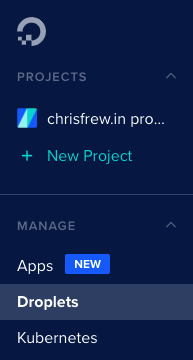
\includegraphics[width=\textwidth/3]{droplet/droplets-tab}
\end{center}

In the new page that opens, click the big green 'Create Droplet' button:

\begin{center}
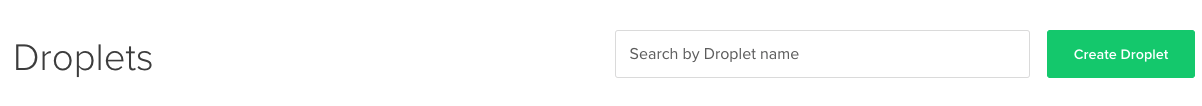
\includegraphics[width=\textwidth]{droplet/new-droplet}
\end{center}

On the resulting page, choose the following settings:

\begin{arrows}
\item Image > Distributions > Ubuntu 20.04 (LTS) x64
\item Plan > Shared CPU > Basic
\item CPU Options > Regular Intel with SSD > \$5 / month
\item Datacenter Region > Choose the option that is closet to where you think most of your customers will be!
\item Authentication > SSH Keys > If you have an SSH key registered, that's great. If not read on below.
\item Choose a hostname > Pick a hostname that matches your project. Of course following the name convention of this book I will be using \codeword{redux-plate}
\end{arrows}

\minisec{Generating a New SSH Key}

If you don't have an SSH key saved with Digital Ocean yet, no worries. Click the 'New SSH Key' button.

So, our Digital Ocean Droplet is spooled up and runs at the insane price of just \$5 / month! Don't think our app will be able to run on such a tiny little instance? Just wait and see!

\section{Using Secrets}

Secret keeping is always a major disussion when it comes to production environments. To handle our app secrets like our PostgreSQL connection string, we'll be using. SOMETHING


\chapter{Payment Integrations}\label{cap:primer}

\section{Introduction}

Payment integrations are of course an essential part of any SaaS production. In this chapter, we'll learn how to connect Stripe, PayPal, and Gumroad into the frontend flow, be notified of both new subscriptions and unsubscriptions, and automatically update the role in the user's netlify Identity user automatically.

\chapter{Building a Staging (or Testing) Environment}\label{cap:primer}

So far we've focused on building out the frontend and custom backend API for ReduxPlate. We write code in our \codeword{develop} git branch, but every time we merge to the \codeword{master} branch in either our frontend or backend repositories, the continuous integration process is fired off and shipped to our live SaaS product immediately. Our continuos integration tool for the frontend is Netlify, and with the backend it is Bitbucket pipelines. That's been great so far for prototyping our MVP, but it's fairly risky once we start having customers.

In this section of the book, we'll get into building out what is known as a staging environment. With all of the tooling available in netlify on the frontend side, and .NET on the backend side, the challenge is not too great, but there will be some important considerations and distinctions which we'll look at in detail.

\section{A Testing Environment is Essential!}\label{sec:titles}

A staging environment is important, because it mimics your live product almost exactly. As we'll see in this section, in comparison to your live product, the staging version of your product will differ only in small configuration changes. Perhaps the exact quality of what certain API endpoints return may differ, but other than that, your staging site is essentially a production-like, risk-free playground where you can test new features, or catch bugs before they ship to production.

\section{Staging CI / CD for the Frontend}\label{sec:titles}

We'll get the client side of things out of the way first. Again, Netlify's powers come to the rescue and setting up a staging version of the frontend is absolute peanuts. 

\section{Create a Staging Branch for the Frontend}\label{sec:titles}

To get started, we'll branch off our develop branch into a new:

\section{Configure Netlify to Build According to the Staging Branch}\label{sec:titles}

On Netlify, head to your product's DNS.

The staging site is up and running! We've got the correct staging environment variables up, builds are firing when we merge to staging; all is well. But if we open a console while looking - we can see . We're getting a bunch of 404 errors when we try to call the staging API endpoint we defined at staging.api.reduxplate.com. Let's switch gears into backend mode and rectify this issue.

\section{Staging CI / CD for the Backend}\label{sec:titles}

Our .NET application will unfortunately be a bit more involved than what it took with Netlify due to it's custom nature. But, .NET and BitBucket offer a lot of powerful features which make the process not too difficult.

\section{Create a Staging Branch for the Backend}\label{sec:titles}

As we did with the frontend, branch of of the development repository for the backend:



\chapter*{Afterword}\label{cap:primer}
\addcontentsline{toc}{chapter}{Afterword}

\section{You've Done It!}\label{sec:titles}

Well, that was quite an adventure. We've both made it out alive! I hope you've found this book immensely useful, and that you're ready to refine your SaaS building skills even further.

\end{document}
